\section{Performance}
\label{sec:performance}

A framework can be fast in two senses: the same model code runs faster on it, or it lets a
modeller write the same model in a faster form. We measure both, with methods chosen to make
the comparison fair and repeatable, and check separately that the faster forms compute the
same model. All the comparisons with Mesa are CPU time (\code{time.process\_time}), measured
in-process, pinned to one core with \code{taskset}, with the implementations alternating, on an
Intel Core Ultra 7 356H laptop running Linux, CPython 3.15.1 for the main timings (3.15.0 for mesa-frames; 3.15.2 for the ablation, the
interpreter comparison and the sweep) and
numpy 2.5.4 in each implementation's environment, against Mesa 2.3.2 and Mesa 3.5.1, with
\modelly{} at its tagged release v1.4.2 (commit \code{bf7a225}); \cref{tab:playbooks} comes from
the second of two timing sessions, whose \code{modelly} package is the tag's
(\cref{app:reproduce}). The core was held at its 1.9~GHz
base frequency (the \code{performance} governor, turbo disabled) for every timing of this
section. Following
\citet{kalibera2013rigorous}, every timed run of the playbooks, the migrated models and Mesa's examples is
a fresh interpreter (the GPU arms are fresh interpreters after one warm-up run), the rounds are
paired and their order varies, and we report medians with their spread and bootstrap intervals
rather than single runs.

\paragraph{Speed-up.} For a workload with CPU times $T_{r}$ over rounds $r = 1, \dots, R$, we
report
\begin{equation}
  S_{\mathrm{steps}} = \frac{\operatorname{median}_r T^{\mathrm{Mesa}}_{\mathrm{steps},r}}
  {\operatorname{median}_r T^{\mathrm{Modelly}}_{\mathrm{steps},r}},
  \qquad
  S_{\mathrm{total}} = \frac{\operatorname{median}_r T^{\mathrm{Mesa}}_{\mathrm{build},r}
  + \operatorname{median}_r T^{\mathrm{Mesa}}_{\mathrm{steps},r}}
  {\operatorname{median}_r T^{\mathrm{Modelly}}_{\mathrm{build},r}
  + \operatorname{median}_r T^{\mathrm{Modelly}}_{\mathrm{steps},r}},
  \label{eq:speedup}
\end{equation}
where \emph{steps} is the simulation and \emph{build} the construction of the model and its
agents. $S_{\mathrm{steps}}$ is the gain per simulated step, which dominates long runs;
$S_{\mathrm{total}}$ is the gain for one run of the benchmark's length. Round $r$ runs every
implementation on seed $r$, so the per-round ratios are paired. Where runs are paired chunk by chunk or round by round
(\cref{sec:samecode,tab:mesa-examples,sec:gpu}) we report instead the
median of the per-round ratios with its range or quartiles; on the playbooks the two
estimators differ by at most 1.6\%.

\subsection{The same model code on both frameworks}
\label{sec:samecode}

\modelly{} shares no code with Mesa; what the two share is a
programming model, so a model written for Mesa can run on \modelly{} once its calls to the
framework are rewritten. \modelly{}'s codemod (\cmd{python -m modelly.migrate}) rewrites a Mesa
model's imports, its agent constructors and the old scheduler calls (\code{schedule.agents},
\code{schedule.steps}, \code{schedule.step()}), leaving every line of model logic unchanged, and
reports the steps it cannot make (the seeding keyword, \code{unique\_id} parameters, schedulers,
legacy grids). The model code is then the same on both frameworks, and the difference in time
is the difference between the frameworks' own calls. We measured it in three settings,
beginning with models we did not write.

\paragraph{Mesa's own examples.} Mesa~3.5 ships ten example models written by its
developers. We migrated copies of them with the codemod, kept in
\code{benchmarks/mesa\_examples/}: eight run on \modelly{} after the codemod and one more edit
to each, the import of the example's own agents made relative (the codemod points it at
\modelly{}'s bundled example of the same name; the relative import makes each copy load the
agents module next to it), plus, for the Epstein civil-violence model, the
one step its report asks for (\code{self.steps} becomes \code{self.time}); Sugarscape G1MT uses
Mesa's property layers and alliance formation its meta-agent factory, which \modelly{} lacks.
The codemod maps Mesa~3.5's module paths, the experimental cell space, continuous space,
meta-agents, signals, scenarios and data collection among them, and reports the other
\code{mesa.experimental} modules and the property-layer module, which \modelly{} lacks; the timed code does not import the
codemod. We ran each original on Mesa and its migrated copy on \modelly{} at Mesa's default
parameters, except four whose defaults run too briefly to time reliably: Boltzmann wealth with
2,500 agents on a $50 \times 50$ grid, Schelling's model on $50 \times 50$, wolf--sheep on
$50 \times 50$ with 625 sheep and 312 wolves, and the virus model on 1,000 nodes
(\code{benchmarks/mesa\_examples/run.py}), each for ten alternating rounds on the same
fixed-frequency core, and compared every model reporter, at the last step and averaged over
the run, over 100 shared seeds. \Cref{tab:mesa-examples} gives the results: on \modelly{} the
examples take 0.60 (wolf--sheep) to 0.95 (the prisoner's dilemma grid and boid flockers) of
Mesa~3.5's CPU time, and all 35 statistics (34 once the virus model's final number infected, zero in every run,
is set aside) are equivalent within $0.5\,s_p$, with no paired $t$-test or
Kolmogorov--Smirnov test below 5\% even before correction. The virus model's other seven
statistics leaned the same way ($|d| = 0.22$ to $0.25$, paired $p \ge 0.10$), and we traced it
(\code{paper/scripts/virus\_trace.py}, \code{data/virus\_trace.json}, 10 seeds): the graph, the
agents' order and neighbourhoods and the data collection are identical on both arms, and only
the initial outbreak differs, because Mesa seeds \code{model.random} with the seed itself and
\modelly{} with a 32-bit value derived from it. With Mesa's derivation forced on both arms the
whole runs are bit-identical on every seed: the migrated copy is the same stochastic process,
draw for draw, and the agreement study compares two independent streams of it. Exact,
run-for-run reproduction of a Mesa model therefore requires aligned random streams: by default
a migrated model draws \code{model.random} from \modelly{}'s seed derivation and agrees with
Mesa in distribution, not run by run. A replication
on 1,000 new seeds (20,000 to 20,999, \code{paper/data/mesa\_examples\_virus1000\_new.json})
gives every $|d| \le 0.016$ (paired $p \ge 0.73$). Here, as for the grid epidemic's peak time
and Schelling's model in \cref{sec:agreement}, a replication on new seeds was run where a
consistent pattern or an interval excluding zero appeared; the other comparisons were not
replicated.

\begin{table}[tbp]
  \centering
  \small
  \caption{Mesa~3.5's own examples on Mesa and, migrated by the codemod, on \modelly{}: median
  CPU time of the steps over ten alternating rounds, \modelly{}'s ratio and its per-round
  range, and the agreement of the model reporters over 100 shared seeds (statistics compared,
  equivalent within $0.5\,s_p$ by paired TOST, lowest Holm-corrected paired $p$). The script
  \code{paper/scripts/mesa\_examples\_table.py} generates it from \code{data/mesa\_examples.json}.}
  \label{tab:mesa-examples}
  \setlength{\tabcolsep}{4pt}
  \begin{tabular}{lrrrrlrrr}
\toprule
 & & \multicolumn{2}{c}{steps (s)} & \multicolumn{2}{c}{port / Mesa} & \multicolumn{3}{c}{agreement} \\
\cmidrule(lr){3-4}\cmidrule(lr){5-6}\cmidrule(lr){7-9}
Example & Steps & Mesa & port & median & range & stats & equiv. & min $p_{\mathrm{Holm}}$ \\
\midrule
Conway's Game of Life & 100 & 0.468 & 0.429 & 0.91 & 0.89--0.94 & 1 & 1/1 & 1.00 \\
Prisoner's dilemma grid & 100 & 1.132 & 1.077 & 0.95 & 0.89--1.02 & 2 & 2/2 & 1.00 \\
Virus on a network & 200 & 0.161 & 0.118 & 0.73 & 0.72--0.75 & 8 & 8/8 & 1.00 \\
Boid flockers & 100 & 0.527 & 0.501 & 0.95 & 0.94--0.96 & 2 & 2/2 & 1.00 \\
Boltzmann wealth & 100 & 0.928 & 0.646 & 0.70 & 0.69--0.71 & 2 & 2/2 & 1.00 \\
Schelling & 50 & 0.249 & 0.177 & 0.71 & 0.69--0.73 & 8 & 8/8 & 1.00 \\
Wolf--sheep & 100 & 0.237 & 0.142 & 0.60 & 0.57--0.63 & 6 & 6/6 & 1.00 \\
Epstein civil violence & 100 & 3.029 & 2.643 & 0.87 & 0.85--1.00 & 6 & 6/6 & 1.00 \\
Sugarscape G1MT & \multicolumn{8}{l}{does not port} \\
Alliance formation & \multicolumn{8}{l}{does not port} \\
\bottomrule
\end{tabular}

\end{table}

\paragraph{Two Mesa~2.3 models.} We also migrated our own Mesa~2.3 implementations of the two
playbooks of \cref{sec:playbooks} that use no Mesa~2 grid (\modelly{} provides cell spaces
instead, so a model on a Mesa~2 grid needs its space rewritten): the insect population and
Boltzmann wealth. The codemod rewrote imports and constructors; the three steps it reported
were done by hand, as its report says (the agents' \code{unique\_id}, the seeding keyword and,
for Boltzmann wealth, the activation order). On \modelly{} (\code{benchmarks/migrated\_mesa2/})
these models give the same statistics as on Mesa~2.3 on every seed tried (20 at the small size, 5 at
the large), and over ten alternating rounds in fresh interpreters on one performance core they
take 0.21 (insect population) and 0.37 (Boltzmann wealth) of Mesa~2.3's CPU time, every round
within 0.20 to 0.22 and 0.37 to 0.38 (\code{paper/scripts/migrated.py}): these models spend
most of their time in framework calls (Mesa~2.3 rebuilds its agent set each time
\code{model.agents} is read and collects agent data in a Python loop), and on \modelly{} those
calls are its compiled ones; upgrading the same models to Mesa~3.5 instead gives 1.9 and 1.8
times (\cref{tab:playbooks}). Models built on a Mesa~2 grid need their space rewritten before
they run on \modelly{}, and their migration was not evaluated.

\paragraph{Five Mesa~3.5 models.} Code written for current Mesa migrates with less effort:
five of the eight Mesa~3.5 playbooks run on \modelly{} after the codemod alone, with no manual
step (\code{benchmarks/migrated\_mesa3/}). The other three do not: flocking uses Mesa's legacy
\code{mesa.space.ContinuousSpace}, and predator-prey and Sugarscape use Mesa~3.5's
\code{PropertyLayer} class, neither of whose APIs \modelly{} reproduces (its own continuous
space has another API, and its property layers are plain \code{numpy} arrays). On \modelly{}
the five take 0.44 (Boltzmann wealth), 0.53 (insect population), 0.73 (grid epidemic), 0.85
(network contagion) and 0.91 (Schelling's model) of Mesa~3.5's CPU time, medians of ten
alternating rounds whose per-round ratios span 0.43--0.45, 0.47--0.58, 0.69--0.76, 0.79--0.91
and 0.89--0.94. Their outputs are not bit-identical to Mesa~3.5's, because \modelly{} derives
\code{model.random} from the seed in a different way, so we compared them in distribution as
in \cref{sec:agreement}: over 100 shared seeds at the small size, 24 of the 26 statistics are
equivalent within $0.5\,s_p$, two paired $t$-tests fall below 5\% before correction (the
network's peak of infections and the Boltzmann model's largest wealth, $|d| \le 0.31$) and
none after it, and no Kolmogorov--Smirnov test does.

The same model code therefore runs 1.05 to 1.7 times faster on \modelly{} for Mesa~3.5's own
examples, 1.1 to 2.3 times for the Mesa~3.5 playbooks, and 2.7 and 4.8 times for the two
Mesa~2.3 models, whose framework calls are slower; the larger gains come from the forms of
\cref{sec:playbooks}.

\subsection{Each framework's own idiom: eight playbooks}
\label{sec:playbooks}

Eight workloads, chosen to exercise different parts of an ABM framework, are each implemented
at least twice: a susceptible--infected--recovered (SIR) epidemic on a grid, predator-prey with grass, flocking
\citep{reynolds1987flocks}, a contagion on a network, a stage-structured insect population,
Schelling's segregation model \citep{schelling1971dynamic}, Boltzmann wealth exchange
\citep{dragulescu2000statistical} and Sugarscape \citep{epstein1996growing}. Each has two
reference implementations written the way Mesa's API intends: one for Mesa~2.3 (per-agent
methods on its grids, continuous space and network space) and one for the current Mesa~3.5
(its cell spaces, \code{CellAgent}, \code{AgentSet.shuffle\_do} and its network space, as in
Mesa's own examples; \cref{app:workloads} notes the choices made), both plain per-agent
Python. Four workloads (the grid epidemic, Schelling's model,
Boltzmann wealth and Sugarscape) also have a \emph{mesa-frames} implementation
\citep{mesaframes}, vectorised over polars data frames the way that library's examples write
models: it is the vectorised Python competitor to \modelly{}'s columns. Three workloads (the
grid epidemic, Schelling's model and Boltzmann wealth) have a \emph{Mesa~3.5 + numpy}
implementation, the hand-vectorised baseline: a \code{mesa.Model} that owns the population as
numpy arrays, with no \code{Agent} objects, and keeps Mesa's grid for its neighbour table and
property layers and Mesa's \code{DataCollector} for the records. It is what an expert gets by
giving up agent objects altogether, and so a reference point for what a framework that keeps them
can reach. Flocking also has a \emph{Mesa~3.5 + KD-tree} implementation, Mesa~3.5's model with
its neighbour search replaced by one periodic \code{scipy.spatial.cKDTree} per step, which
separates the algorithm from the framework (\cref{sec:threats}). The \modelly{}
implementation uses column state, \code{CellIndex}, KD-tree queries or cohorts, and four
workloads have a further \modelly{} variant, \emph{cell lists}, which keeps per-cell
agent lists and vectorises only the obvious phases (\cref{app:workloads}). The
implementations agree within the margins that \cref{sec:agreement} measures and reports,
apart from a small shift in our mesa-frames Schelling implementation (under 1\% of the mean;
\cref{sec:agreement}), and three Mesa~3.5
implementations, which draw the same random numbers in the same order as Mesa~2.3, reproduce
it run by run: flocking, the network contagion and the insect population. Each implementation
is run twice from the same seed and must reproduce its own output exactly; all do.
\Cref{tab:workloads} in the appendix gives every workload's parameters. All variants of all
workloads were timed in one session, ten rounds each, and again in a second session that
agrees with it within 4\% on every speed-up (\cref{sec:threats}), on one performance core, the order of
the variants rotating from round to round; each result file records the commit, the date, the
load, the core and its power policy, and every package version. \Cref{sec:threats} gives the
per-round spreads and the load during the session, and \cref{tab:speedup-ci} in the appendix a
bootstrap 95\% interval for every speed-up, resampling the paired rounds.

\begin{table}[tbp]
  \centering
  \small
  \caption{The playbooks at their large size: median CPU time of building the model and of
  running its steps over ten rounds, the speed-ups of \cref{eq:speedup} over Mesa~2.3, and the
  speed-up of the steps over Mesa~3.5; \cref{tab:speedup-ci} gives their 95\% intervals. Agents:
  the population at the end of the last round. The GPU variants of the grid epidemic and the
  insect population, timed in the same session on the CPU, are left out: they draw from Philox
  streams and are reported with the GPU (\cref{sec:gpu}); on the CPU the grid epidemic's GPU
  variant runs its steps in 0.114~s against the columns' 0.155~s. Generated from
  \code{benchmarks/playbooks/results/} by \code{paper/scripts/make\_figures.py}.}
  \label{tab:playbooks}
  \setlength{\tabcolsep}{4.5pt}
  \begin{tabular}{llrrrrrr}
\toprule
 & & & \multicolumn{2}{c}{CPU time (s)} & \multicolumn{2}{c}{over Mesa 2.3} & over Mesa 3.5 \\
\cmidrule(lr){4-5}\cmidrule(lr){6-7}\cmidrule(lr){8-8}
Workload & Variant & Agents & build & steps & steps & total & steps \\
\midrule
Grid epidemic (SIR) & Mesa 2.3 & 20{,}000 & 0.035 & 7.098 & 1.0 & 1.0 & -- \\
 & Mesa 3.5 & 20{,}000 & 0.339 & 4.311 & 1.6 & 1.5 & -- \\
 & Mesa 3.5 + numpy & 20{,}000 & 0.299 & 0.035 & 200.2 & 21.3 & 121.6 \\
 & mesa-frames & 20{,}000 & 0.017 & 1.098 & 6.5 & 6.4 & 3.9 \\
 & Modelly, cell lists & 20{,}000 & 0.154 & 2.872 & 2.5 & 2.4 & 1.5 \\
 & Modelly, columns & 20{,}000 & 0.167 & 0.157 & 45.3 & 22.0 & 27.5 \\
\addlinespace
Predator-prey & Mesa 2.3 & 5{,}421 & 0.008 & 3.385 & 1.0 & 1.0 & -- \\
 & Mesa 3.5 & 5{,}453 & 0.310 & 3.729 & 0.9 & 0.8 & -- \\
 & Modelly, cell lists & 5{,}567 & 0.125 & 2.188 & 1.5 & 1.5 & 1.7 \\
 & Modelly, columns & 5{,}402 & 0.124 & 0.526 & 6.4 & 5.2 & 7.1 \\
\addlinespace
Flocking (boids) & Mesa 2.3 & 4{,}000 & 0.015 & 24.578 & 1.0 & 1.0 & -- \\
 & Mesa 3.5 & 4{,}000 & 0.023 & 24.661 & 1.0 & 1.0 & -- \\
 & Modelly, columns & 4{,}000 & 0.018 & 0.749 & 32.8 & 32.1 & 32.9 \\
\addlinespace
Network contagion & Mesa 2.3 & 30{,}000 & 0.174 & 7.807 & 1.0 & 1.0 & -- \\
 & Mesa 3.5 & 30{,}000 & 0.434 & 2.511 & 3.1 & 2.7 & -- \\
 & Modelly, columns & 30{,}000 & 0.600 & 0.199 & 39.3 & 10.0 & 12.6 \\
\addlinespace
Insect population & Mesa 2.3 & 27{,}233 & 0.001 & 3.674 & 1.0 & 1.0 & -- \\
 & Mesa 3.5 & 27{,}233 & 0.002 & 2.007 & 1.8 & 1.8 & -- \\
 & Modelly, columns & 27{,}042 & 0.002 & 0.684 & 5.4 & 5.4 & 2.9 \\
 & Modelly, cohorts & 26{,}465 & 0.002 & 0.015 & 243.3 & 217.4 & 132.9 \\
\addlinespace
Schelling segregation & Mesa 2.3 & 31{,}951 & 0.044 & 4.646 & 1.0 & 1.0 & -- \\
 & Mesa 3.5 & 32{,}068 & 0.380 & 3.580 & 1.3 & 1.2 & -- \\
 & Mesa 3.5 + numpy & 31{,}951 & 0.354 & 0.116 & 40.0 & 10.0 & 30.9 \\
 & mesa-frames & 31{,}951 & 0.020 & 1.925 & 2.4 & 2.4 & 1.9 \\
 & Modelly, cell lists & 31{,}951 & 0.255 & 0.323 & 14.4 & 8.1 & 11.1 \\
 & Modelly, columns & 31{,}951 & 0.302 & 0.205 & 22.7 & 9.3 & 17.5 \\
\addlinespace
Boltzmann wealth & Mesa 2.3 & 10{,}000 & 0.009 & 2.138 & 1.0 & 1.0 & -- \\
 & Mesa 3.5 & 10{,}000 & 0.024 & 1.136 & 1.9 & 1.9 & -- \\
 & Mesa 3.5 + numpy & 10{,}000 & $<$0.001 & 0.121 & 17.6 & 17.6 & 9.4 \\
 & mesa-frames & 10{,}000 & 0.006 & 0.997 & 2.1 & 2.1 & 1.1 \\
 & Modelly, columns & 10{,}000 & 0.026 & 0.335 & 6.4 & 5.9 & 3.4 \\
\addlinespace
Sugarscape & Mesa 2.3 & 710 & 0.004 & 1.490 & 1.0 & 1.0 & -- \\
 & Mesa 3.5 & 702 & 0.043 & 1.455 & 1.0 & 1.0 & -- \\
 & mesa-frames & 715 & 0.013 & 2.104 & 0.7 & 0.7 & 0.7 \\
 & Modelly, cell lists & 703 & 0.028 & 1.133 & 1.3 & 1.3 & 1.3 \\
 & Modelly, columns & 712 & 0.045 & 0.325 & 4.6 & 4.0 & 4.5 \\
\bottomrule
\end{tabular}

\end{table}

\begin{figure}[tbp]
  \centering
  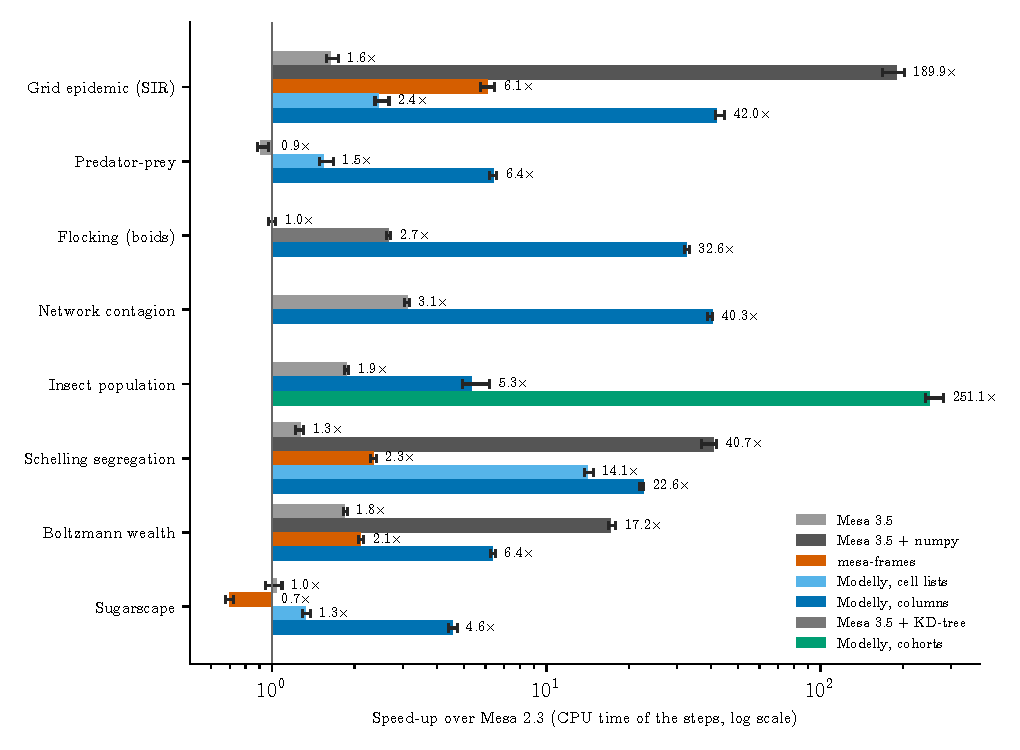
\includegraphics[width=\linewidth]{figures/speedups}
  \caption{$S_{\mathrm{steps}}$ of each implementation over the Mesa~2.3
  implementation of the same workload (\cref{tab:playbooks}); whiskers span the per-round
  ratios, and bars left of 1 are slower than Mesa~2.3. Columns and cohorts are \modelly{}'s
  array-based storage; cell lists keep per-cell agent lists, as Mesa's grids do; mesa-frames is the vectorised
  data-frame library built on Mesa; Mesa~3.5 + numpy replaces Mesa's agents with hand-written
  arrays.}
  \label{fig:speedups}
\end{figure}

\paragraph{Where \modelly{} is fast, and why.} \modelly{}'s column form runs every workload
faster than Mesa~2.3 and Mesa~3.5, and faster than mesa-frames on the four it implements
(\cref{tab:playbooks,fig:speedups}): its steps run
4.6 to 42 times faster than Mesa~2.3, 2.9 to 33 times faster than Mesa~3.5 and 3.0 to 9.6 times
faster than mesa-frames, and its cohort form runs the insect population 251 times faster than
Mesa~2.3 and 135 times faster than Mesa~3.5. \Cref{tab:why} gives the reason workload by
workload. In each, one \modelly{} mechanism replaces a Python loop over the agents with a few
array operations over the whole population: a column read or write instead of an attribute per
agent, one count over the grid's adjacency instead of a neighbourhood walk per agent, one
KD-tree query instead of a distance test per pair, one sparse product over a network instead of
a loop over each node's neighbours, one binomial draw per class instead of one draw per insect.
The gain therefore grows with the share of a step that such a mechanism covers: largest where
every phase becomes array work (flocking, the grid epidemic, Schelling's model, the network),
smaller where a phase must stay sequential, as the foragers' walk to a free cell in Sugarscape,
or where the step creates and removes many agents, as the births and deaths of predator-prey
and of the individual insect model, or where a cost every implementation shares dominates the
step, as Boltzmann wealth's data collector, which records the Gini coefficient and every
agent's wealth after each step (\cref{sec:threats}). Code that gives up agent objects
altogether goes further still: hand-written numpy is 1.8 to 4.5 times faster than the columns
(below). The arguments that each vectorised phase has the law of its
per-agent loop are given in the documentation (\code{docs/vectorised\_phases.md}), and
\cref{sec:agreement} checks that the outputs agree.

\begin{table}[tbp]
  \centering
  \small
  \caption{Where \modelly{}'s speed comes from: for each workload, from the largest step-time
  speed-up over Mesa~2.3 in \cref{tab:playbooks} to the smallest (the insect population by its
  cohort form), the mechanism that replaces the per-agent
  Python loop, as the code of each implementation shows (the attribution comes from the code,
  not from per-workload profiles).}
  \label{tab:why}
  \begin{tabularx}{\linewidth}{@{}l >{\raggedright\arraybackslash}X@{}}
    \toprule
    Workload & What \modelly{} does instead of a loop over agents \\
    \midrule
    Insect population & cohorts: at most about 190 (stage, age, sex) classes thinned by
      binomial draws replace about 26,000 agents \\
    Grid epidemic & positions are a column of cells: the walk is one \code{random\_neighbor}
      call, the exposure one count of infected per cell \\
    Network contagion & infected neighbours of every node in one sparse matrix--vector
      product; infection and recovery are Bernoulli vectors \\
    Flocking & one periodic KD-tree query for the whole flock; the steering terms are pair sums
      scattered back with \code{bincount}; positions written in one call \\
    Schelling & happiness is two sparse products (residents per cell, summed over neighbours);
      all moves in one pass with the sequential rule's law \\
    Predator-prey & movement, energy, grazing and predation (\code{claim}) are array
      operations; deaths and births are one call per species \\
    Boltzmann wealth & the exchange is a few array passes (a fixed-point iteration) with the
      law of the shuffled sequential order \\
    Sugarscape & every forager's best visible cell found in one array pass; only the walk to
      a free cell stays sequential \\
    \bottomrule
  \end{tabularx}
\end{table}

\paragraph{The other implementations.} Mesa~3.5 is faster than Mesa~2.3 on five workloads
(1.3 to 3.1 times), as fast on flocking and Sugarscape, and slower on predator-prey (0.91
times). mesa-frames is 2.1 to 6.1 times faster than Mesa~2.3 on three of its four workloads and
slower on Sugarscape (0.70 times), where its per-forager search is a cross join and a sort over
up to about 130,000 rows per step. \modelly{}'s cell-list variants, which keep per-cell
agent lists, give 1.3 to 14 times over Mesa~2.3 and 1.3 to 11 over Mesa~3.5: large for
Schelling's model, whose residents mostly count their neighbours, small where movement and
search stay per agent. Construction is where \modelly{} spends more than Mesa~2.3 (it
allocates the columns and indexes the space; Mesa~3.5's cell spaces cost about as much, 0.31
to 0.43~s on the three large grids and the network), so the column form's gain including construction is
4.0 to 32 times, and lower than per step on short runs such as the network contagion (40 times
per step, 10 in total).

\paragraph{Against hand-written numpy.} The Mesa~3.5 + numpy baseline is faster than
\modelly{}'s columns on all three of its workloads: its steps take 0.034~s against 0.155~s on
the grid epidemic (4.5 times faster, 95\% interval 4.1 to 4.6), 0.112~s against 0.201~s on
Schelling's model (1.8 times, 1.8 to 1.8) and 0.121~s against 0.328~s on Boltzmann wealth (2.7
times, 2.7 to 2.7; there partly because it records the wealth as one array per step rather than
as per-agent rows). It pays for that with the model's structure: no agent has an identity,
methods or attributes of its own, the population cannot hold agents of several kinds, every
neighbourhood is a hand-built index table, and every phase has to be rewritten as array
operations before the model runs at all, whereas \modelly{} keeps agent objects, agent sets and
spaces next to the columns, and lets a model be vectorised one phase at a time. Its agreement
with Mesa~2.3 is that of the other implementations (\cref{tab:agreement-mesa3np}: 13 of 14
statistics equivalent within $0.5\,s_p$); the one paired $t$-test below 5\% after the Holm
correction is Schelling's segregation ($d = 0.24$, 0.6\% of the mean). The baseline runs the
column algorithm without the framework layer, and on these seeds its Schelling and Boltzmann
wealth runs give exactly the column variant's statistics, so the two share this difference
and any bias behind it; on 300 new seeds the column variant's segregation has $d = 0.07$
$[-0.02, 0.15]$ (\cref{tab:agreement-schelling300}). The benchmark harness's own six-seed
check flags three of its six grid epidemic statistics, flags that vanish over 100 seeds (at the
small size lowest paired $p$ 0.13 and largest $|d|$ 0.21; at the timed size 0.19 and 0.20;
all six equivalent in both; \code{paper/data/agreement\_large\_grid\_mesa3np.json}). The gap is the price of the
framework layer: \modelly{} sits between per-agent Mesa and hand-written arrays,
3.5 to 26 times above Mesa~3.5 and 1.8 to 4.5 times below the numpy baseline on these three workloads.

\paragraph{How the gain changes with population size.} The playbooks are timed at one size;
\cref{tab:sizes} times three of them, whose populations scale with one parameter, at the
playbook's small size, its timed size and ten times that, five rounds each on the same
fixed-frequency core (\code{paper/scripts/sizes.py}, \code{paper/data/sizes.json}). On the
grid epidemic and Schelling's model the columns' lead grows with the population: on the grid
epidemic it goes from 4.0 to 42 and 119
times over Mesa~2.3 and from 2.4 to 26 and 67 times over Mesa~3.5 as the population goes from
2,000 to 20,000 and 200,000 agents; on Schelling's model from 1.3 to 22 and 44 times over
Mesa~2.3 and from 1.0 to 18 and 32 times over Mesa~3.5; on Boltzmann wealth, whose data
collector records every agent's wealth each step, it grows over Mesa~2.3 (4.0, 6.4 and 10
times) but stays at 2.8 to 3.6 times over Mesa~3.5, and shrinks over mesa-frames (14, 3.0 and
2.0 times). At the smallest sizes the framework's fixed cost per step weighs most: on Schelling's model with
1,282 residents the columns are as fast as Mesa~3.5. Hand-written numpy's lead over the columns
shrinks the other way on the grid epidemic (17, 4.6 and 1.6 times) and Schelling's model (13.5,
1.8 and 1.0 times), where at large populations the columns run at nearly the speed of code
without agents while keeping them; on Boltzmann wealth it stays at 1.9 to 2.8 times.

\begin{table}[tbp]
  \centering
  \small
  \caption{The step-time speed-ups of \modelly{}'s columns, and of hand-written numpy over the
  columns, at three population sizes: the playbook's small size, its timed size (as in
  \cref{tab:playbooks}) and ten times that at the same density. Medians of five rotated rounds
  on one fixed-frequency core; agents at the end of the run. Generated by
  \code{paper/scripts/sizes.py}.}
  \label{tab:sizes}
  \setlength{\tabcolsep}{4pt}
  \begin{tabular}{llrrrrrr}
\toprule
 & & & & \multicolumn{3}{c}{columns faster than} & numpy faster \\ \cmidrule(lr){5-7} Workload & Size & Agents & Mesa 2.3, s & Mesa 2.3 & Mesa 3.5 & mesa-frames & than columns \\
\midrule
Grid epidemic & small & 2{,}000 & 0.40 & 4.0 & 2.4 & 2.6 & 17.0 \\
 & large & 20{,}000 & 6.50 & 42.2 & 25.9 & 6.9 & 4.6 \\
 & huge & 200{,}000 & 95.49 & 119 & 66.6 & 12.6 & 1.6 \\
\addlinespace
Schelling & small & 1{,}282 & 0.13 & 1.3 & 1.0 & 2.6 & 13.5 \\
 & large & 32{,}090 & 4.50 & 22.4 & 17.9 & 9.6 & 1.8 \\
 & huge & 319{,}610 & 58.69 & 43.9 & 32.1 & 16.9 & 1.0 \\
\addlinespace
Boltzmann wealth & small & 500 & 0.08 & 4.0 & 2.8 & 14.1 & 1.9 \\
 & large & 10{,}000 & 2.10 & 6.4 & 3.5 & 3.0 & 2.7 \\
 & huge & 100{,}000 & 41.33 & 10.2 & 3.6 & 2.0 & 2.8 \\
\bottomrule
\end{tabular}

\end{table}

\paragraph{On other interpreters.}
\label{sec:python-versions}
Every timing above ran on CPython~3.15. Since per-agent code gains from each interpreter
release and array code does not, the ratios could depend on the version, so we timed the
Mesa~3.5 and column implementations of all eight playbooks (and the insect population's
cohorts) under CPython 3.12, 3.14 and 3.15, each in its own environment with the same
package versions and \modelly{}'s C modules built for it, five rotated rounds in fresh
interpreters pinned to one core at the machine's default frequency policy
(\code{paper/scripts/python\_versions.py}, \cref{tab:python-versions} in the appendix). The
speed-ups on 3.15 reproduce \cref{tab:playbooks}'s within the session's noise (26.1, 7.1,
31.5, 12.9, 3.0, 17.7, 3.5 and 4.4 against 25.7, 7.1, 32.6, 12.9, 2.9, 17.8, 3.5 and 4.4;
the cohorts 135 against 135), and on 3.12 and 3.14 they are similar or larger: 33 and 32
on the grid epidemic, 9.7 and 7.7 on predator-prey, 17 and 22 on Schelling's model, 4.3 and
4.2 on Boltzmann wealth, within 10\% of the 3.15 values on the other four, with the
cohorts at 151 and 159. Mesa's per-agent steps are 1 to 28\% faster on 3.15 than on 3.12
(20\% on the grid epidemic, 28\% on predator-prey) while the columns' steps change by at
most 5\% on six playbooks (16\% on Schelling's model and 14\% on the insect population,
whose column steps keep some per-agent work), so the newest interpreter is the least
favourable of the three to \modelly{} on six of the eight workloads (a tie on the insect
population's columns; Schelling's model 5\% lower on 3.12), and the speed-ups reported in
the paper are, within 5\%, the conservative ones.

\paragraph{A sweep end to end.}
\label{sec:sweep}
Step time dominates long runs; a sweep of short runs also pays for starting workers,
importing and building the model, reading its outputs after every step and writing them
to the store. We timed one small sweep end to end (\code{paper/scripts/sweep\_e2e.py},
\cref{tab:sweep} in the appendix): 64 runs of the grid epidemic at the small size (a
16-point Latin hypercube over $\beta$, four replicates, 60 steps, one output per step), from
the creation of the \code{Experiment} to its results queried from the Parquet store,
driven by \modelly{}'s experiment layer with each of the two engines, the column
implementation and the Mesa~3.5 one (which takes its parameters by name and steps like any
model, so the workflow's overhead is the same on both sides), medians of five rounds in
fresh interpreters. On the serial executor pinned to one core the sweep takes 2.18~s with
the columns and 16.98~s with Mesa~3.5, a factor of 7.8, against 12 for the simulation alone
at this size (0.020 against 0.244~s per run): with runs this short, 40\% of the column
sweep is the workflow (0.014~s per run: the task's dispatch, the output read after each of
the 61 states, the Parquet write) and 8\% of the Mesa one. On four processes the Mesa sweep is 2.4 times faster than serial and
the column sweep no faster (2.20~s): 64 runs of 0.02~s do not repay starting four workers
and importing the model in each, so a sweep of runs this short on \modelly{} should stay
serial, or batch many runs per task. The gain a study sees from the columns is therefore
the step-time speed-up for long runs and, for short runs, a smaller factor that the
workflow's fixed cost per run bounds; \cref{tab:playbooks}'s $S_{\mathrm{total}}$ gives
the bound from construction alone, and this measurement adds the experiment layer's share.
The session ran at the machine's default frequency policy under a load average of 10 to 21
(the fourth round, under the heaviest load, is the slowest in every arm).

\paragraph{mesa-frames with more threads.} polars runs multi-threaded by default, while the
timings above set \code{POLARS\_MAX\_THREADS=1} so that every implementation uses one core;
pinned to the four performance cores, five alternating rounds in wall-clock time, mesa-frames
with four threads was slower than with one on all four of its workloads (Schelling's model
3.41~s against 2.86~s; \code{paper/data/frames\_threads\_pinned.json}), so on those cores the
one-thread comparison does not handicap it. With all 16 threads, unpinned, single runs gave
Schelling's model 1.4 times faster and the other three slower (\cref{app:workloads}): on the
whole machine the one-thread comparison may overstate the columns' lead on Schelling's model
by up to that factor.

\subsection{Where the gain comes from: an ablation}
\label{sec:ablation}

Between per-agent Mesa~3.5 code and \modelly{}'s column form several things change at
once: the framework whose calls the same code makes, whether those calls run in C or in
Python, the data structure that holds the population, the algorithm of a search, and
whether a phase is written per agent or as array operations. To attribute the gain, we timed
a ladder of implementations that changes one of these per rung on four workloads
(\code{paper/scripts/ablation.py}, \cref{tab:ablation}): ten rotated rounds in fresh
interpreters pinned to one core, each \modelly{} rung run twice, once with
\code{MODELLY\_PURE\_PYTHON=1} (the framework's inner loops in Python) and once with the C
modules, so that the compiled runtime's share is read off within the rung. The session ran
at the machine's default frequency policy, so its absolute times differ from
\cref{tab:playbooks} (they are 6 to 19\% shorter); every ratio is paired within the
session, and the speed-ups of the columns over Mesa~3.5 that it gives (26.4, 18.5, 33.5
and 4.5) agree with the main table's (25.7, 17.8, 32.6 and 4.4) within 4\%.

\begin{table}[htbp]
  \centering
  \small
  \caption{The ablation: one ladder of implementations per workload, each rung changing one
  thing from the rung above. Median CPU time of the steps over ten rotated rounds with the
  framework's inner loops in Python (\code{MODELLY\_PURE\_PYTHON=1}) and compiled; the
  compiled runtime's gain within the rung (median of the per-round ratios); and the speed-up
  of the compiled rung over Mesa~3.5 and over the rung above. The Mesa~3.5 and numpy rungs
  have no Python-core arm. Generated by \code{paper/scripts/ablation.py} from
  \code{paper/data/ablation.json}.}
  \label{tab:ablation}
  \setlength{\tabcolsep}{4pt}
  \begin{tabularx}{\linewidth}{l>{\raggedright\arraybackslash}Xrrrrr}
\toprule
 & & \multicolumn{2}{c}{steps (s)} & & \multicolumn{2}{c}{speed-up (compiled)} \\
\cmidrule(lr){3-4}\cmidrule(lr){6-7}
Workload & Rung & Python & compiled & C gain & Mesa~3.5 & rung above \\
\midrule
Grid epidemic & Mesa 3.5: per-agent code on Mesa's cell space & -- & 3.526 & -- & 1.0 & -- \\
 & migrated: same code, Modelly's calls (codemod) & 3.284 & 2.627 & 1.27 & 1.3 & 1.34 \\
 & cell lists: Mesa's data structure; infection phase as arrays & 2.880 & 2.328 & 1.23 & 1.5 & 1.10 \\
 & columns: every phase as arrays over columns & 0.131 & 0.133 & 0.99 & 26.4 & 18.00 \\
 & Mesa 3.5 + numpy: arrays without agent objects or framework & -- & 0.029 & -- & 119.1 & 4.56 \\
\addlinespace
Schelling & Mesa 3.5: per-agent code on Mesa's cell space & -- & 3.367 & -- & 1.0 & -- \\
 & migrated: same code, Modelly's calls (codemod) & 3.239 & 3.110 & 1.04 & 1.1 & 1.10 \\
 & cell lists: Mesa's data structure; neighbour count as arrays & 0.330 & 0.302 & 1.09 & 11.3 & 10.08 \\
 & columns: every phase as arrays over columns & 0.180 & 0.183 & 1.00 & 18.5 & 1.65 \\
 & Mesa 3.5 + numpy: arrays without agent objects or framework & -- & 0.105 & -- & 32.7 & 1.73 \\
\addlinespace
Flocking & Mesa 3.5: per-agent code, all-pairs neighbour scan & -- & 23.039 & -- & 1.0 & -- \\
 & Mesa 3.5 + KD-tree: same code, one KD-tree per step & -- & 8.335 & -- & 2.6 & 2.60 \\
 & columns: KD-tree; steering as arrays over columns & 0.668 & 0.663 & 1.04 & 33.5 & 13.15 \\
\addlinespace
Sugarscape & Mesa 3.5: per-agent code, one search per forager & -- & 1.158 & -- & 1.0 & -- \\
 & cell lists: Mesa's data structure, same search & 0.994 & 0.909 & 1.10 & 1.3 & 1.25 \\
 & columns: search as one array pass over columns & 0.260 & 0.257 & 1.00 & 4.5 & 3.50 \\
\bottomrule
\end{tabularx}
% 10 rounds, core 2

\end{table}

\paragraph{What each rung contributes.} The framework's own calls, with no phase rewritten,
are worth little: the same code migrated to \modelly{} runs 1.06 times faster than on
Mesa~3.5 with the inner loops in Python (grid epidemic and Schelling alike), and the C
modules add a factor of 1.27 on the grid epidemic, whose step is dominated by per-agent
moves and neighbourhood reads that the compiled loops serve, and 1.04 on Schelling's model,
whose step is dominated by neighbour counting in model code. The data structure alone is
worth about as little: on Sugarscape, where the cell-list variant runs Mesa's search
algorithm on \modelly{}'s cell lists, it gives 1.13 with the Python core and 1.25 with the
compiled one. The algorithm is worth what it is worth: the KD-tree alone makes Mesa~3.5's
flocking 2.6 times faster. Everything else is the array form of the phases. On the grid
epidemic, moving from cell lists to columns, with no change of algorithm and with the C
modules off on both sides, is a factor of 22; on Schelling's model vectorising the
neighbour count alone (the cell-list rung, Python core) is a factor of 10 over the migrated
code and vectorising the moves as well (columns) another 1.8; on flocking the steering
terms as array operations are a factor of 12.5 over the KD-tree baseline; on Sugarscape
the search as one array pass is a factor of 3.9 over the same search per forager. The
compiled runtime contributes nothing to the column rungs (0.99 to 1.04): once a phase is an
array operation, the framework's loops are no longer on the path, and the time is numpy's.
In the ablation's session the column form sits 1.7 to 4.6 times above hand-written numpy
without agent objects (1.8 to 4.5 in \cref{tab:playbooks}),
which is the price of keeping agents, agent sets and spaces next to the arrays.
The attribution is therefore: of the grid epidemic's factor of 26, about 1.3 is the
framework and its compiled loops and about 20 the array representation of the phases; of
flocking's 34, 2.6 is the neighbour-search algorithm and 13 the array form of the
steering; of Schelling's 19, 1.1 is the framework and 17 the array form; of Sugarscape's
4.5, 1.25 is the data structure and 3.5 the array form of the search.

\subsection{Do the faster forms compute the same model?}
\label{sec:agreement}

The implementations draw their random numbers in different orders, so their dynamics cannot
agree run by run; they must agree in distribution. Where two implementations draw the initial
state the same way, a seed gives both the same start: strongly in Sugarscape (correlation
between the two implementations' outputs on a seed $r = 0.91$ to $0.99$) and Schelling's model
($0.42$ to $0.70$), completely in flocking, whose dynamics are deterministic once it has
started ($r = 1$). The comparisons are therefore paired, seed by seed. We ran the Mesa~2.3
reference and every \modelly{} variant of every playbook on the same 100 seeds at the playbook's
small size (2,100 runs), and compared each of the 67 pairs of a summary statistic and a \modelly{} variant (epidemic peak
and final size, final populations, cluster counts, Gini coefficient, and so on) with the Mesa
reference in three ways: a paired $t$-test on the seed-by-seed differences, the two-sample
Kolmogorov--Smirnov test on the two marginal distributions (an unpaired test, conservative
here because the shared seeds correlate the samples, and more so for the integer-valued
statistics, whose values tie, so it serves as a coarse check only), and paired two one-sided tests
(TOST) of equivalence \citep{schuirmann1987comparison, lakens2017equivalence} with a margin of
half a pooled standard deviation $s_p$, that is, against the null hypothesis
$|\mu_{\mathrm{Modelly}} - \mu_{\mathrm{Mesa}}| \ge 0.5\, s_p$. We report the standardised
difference $d = (\bar x_{\mathrm{Modelly}} - \bar x_{\mathrm{Mesa}}) / s_p$ with its paired 95\%
interval, and correct for the 67 comparisons with Holm's procedure \citep{holm1979simple}.
\Cref{tab:agreement-all} in the appendix lists every comparison. Three kinds of statement
follow from these tests, and we keep them apart throughout: a comparison is \emph{shown
equivalent} when its TOST rejects at 5\% (nominally, one comparison at a time; or after the
Holm correction, which controls the familywise error over the 67); a comparison is
\emph{shown different} when its paired interval excludes zero; and a comparison that is
neither is \emph{undecided}, not equal, since a nonsignificant difference test can reflect
low power. The margin of $0.5\,s_p$ is a convention (a medium effect by Cohen's scale), not
a scientific tolerance; we therefore also report how the counts change with the margin,
give counts at margins relative to Mesa's mean, and, in \cref{sec:trajectories}, test
science-specific margins prespecified in each quantity's own units.

\begin{table}[htbp]
  \centering
  \small
  \caption{Agreement with Mesa~2.3 over 100 shared seeds per variant, at the small size: the
  largest standardised difference, the lowest paired $t$ and Kolmogorov--Smirnov $p$-values
  (before correction), and the number of statistics equivalent within $0.5\,s_p$ (paired TOST
  at 5\%, uncorrected).
  Generated by \code{paper/scripts/agreement.py}.}
  \label{tab:agreement}
  \begin{tabular}{llrrrrr}
\toprule
Workload & Modelly variant & Stats & max $|d|$ & min $p_{t}$ & min $p_{\mathrm{KS}}$ & Equivalent \\
\midrule
Grid epidemic & cell lists & 6 & 0.23 & 0.08 & 0.15 & 6/6 \\
Grid epidemic & columns & 6 & 0.13 & 0.39 & 0.58 & 6/6 \\
Predator-prey & cell lists & 5 & 0.30 & 0.02 & 0.01 & 4/5 \\
Predator-prey & columns & 5 & 0.13 & 0.34 & 0.47 & 5/5 \\
Flocking & columns & 3 & 0.00 & 0.90 & 1.00 & 3/3 \\
Network contagion & columns & 6 & 0.16 & 0.20 & 0.21 & 6/6 \\
Insect population & columns & 6 & 0.33 & 0.02 & 0.04 & 4/6 \\
Insect population & cohorts & 6 & 0.23 & 0.10 & 0.21 & 6/6 \\
Schelling & cell lists & 4 & 0.23 & 0.03 & 0.37 & 4/4 \\
Schelling & columns & 4 & 0.24 & $<$0.01 & 0.28 & 4/4 \\
Boltzmann wealth & columns & 4 & 0.29 & 0.03 & 0.21 & 3/4 \\
Sugarscape & cell lists & 6 & 0.03 & 0.33 & 0.82 & 6/6 \\
Sugarscape & columns & 6 & 0.01 & 0.65 & 0.97 & 6/6 \\
\bottomrule
\end{tabular}
% 100 seeds per variant

\end{table}

\begin{figure}[htbp]
  \centering
  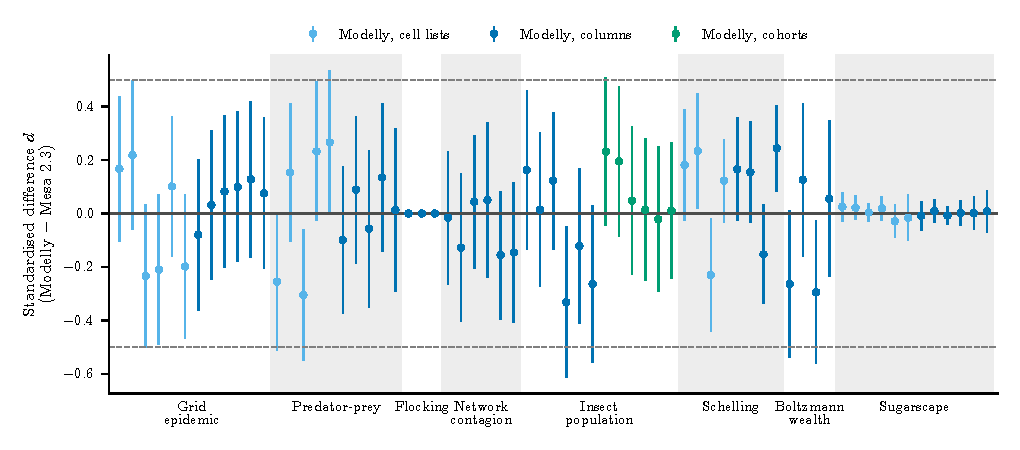
\includegraphics[width=\linewidth]{figures/agreement_small}
  \caption{Standardised difference $d$ between each \modelly{} variant and Mesa~2.3 for every
  summary statistic, with 95\% intervals, over 100 seeds; dashed lines: the equivalence margin
  $\pm 0.5\,s_p$. Flocking is deterministic once its initial state is drawn, and both
  implementations draw it from the same seeded \code{numpy} stream: it agrees run by run to
  rounding error, hence $d = 0$.}
  \label{fig:agreement}
\end{figure}

\Cref{tab:agreement} and \cref{fig:agreement} give the results. Within the margin of
$0.5\,s_p$, 63 of the 67 comparisons are shown equivalent at the nominal 5\% level (60 of 64
outside flocking, whose three agree trivially), and 29 of 67 after the Holm correction of
the TOST $p$-values. The two counts answer different questions: the first says how many
comparisons, each taken on its own, meet the margin; the second how many do so with the
familywise error held at 5\% over all 67, and it is the one to quote when the claim is
about the set. The four comparisons not shown equivalent even nominally are the mean sheep
population of predator-prey with cell lists, the final and the peak adult counts of the
individual insect model, and the share of agents without wealth in the Boltzmann model
($|d| \le 0.33$, at most 1.4\% of the mean). The count depends on the margin: 50 at
$0.4\,s_p$, 27 at $0.3\,s_p$ and 19 at $0.25\,s_p$; with a margin relative to Mesa's mean
instead, 48 of 67 are shown equivalent within $\pm 5\%$ and 56 within $\pm 10\%$, the others
being the noisiest statistics at this small size (the grid epidemic's counts with 2,000
agents, predator-prey's wolves), whose 100-seed intervals are wider than those margins.
The intervals themselves are the most direct summary: every $|d|$ is at most 0.33, 58 of the 67 intervals lie within $[-0.5, 0.5]$ and all
within $[-0.62, 0.62]$; every difference of means is at most 11\% of Mesa's, and under 5\%
for 59 of 67. Six intervals exclude zero, so six differences are shown,
taken one at a time: three in Schelling's model ($|d| \le 0.24$, at most 4.3\% of the
mean, made detectable by the shared initial state), the mean sheep population of
predator-prey with cell lists, the final adult count of the individual insect model and the
share of agents without wealth in the Boltzmann model ($|d| \le 0.33$, at most 1.4\%).
After the Holm correction no paired or Kolmogorov--Smirnov test falls below 5\% (the
smallest corrected paired $p$ is 0.21); we do not read this as equality, since at the
corrected level a paired test on 100 seeds detects $d = 0.33$ with probability 0.13 only
(\cref{sec:threats}), but as consistent with the intervals above. Before correction, six
paired $t$-tests and three Kolmogorov--Smirnov tests fall below 5\%, against 3.2 expected by
chance for each test among the 64 comparisons outside flocking if the tests were
independent (they are not: the statistics of a workload are related, such as its final S, I
and R). The spreads agree too: the ratio of the two implementations' standard deviations
lies between 0.77 and 1.27, and one median-centred Levene test \citep{brown1974robust} of 67
falls below 5\%, none after the Holm correction; within the power of a Levene test on 100
seeds (unpaired, and so conservative here) this is consistent with a vectorised phase
leaving the variability of an outcome unchanged, and no more. The benchmark harness's own
quick check, six seeds and an unpaired Welch test \citep{welch1947generalization} at 1\%,
could not have shown any of this: its power to detect a difference of one standard
deviation is 13\%.

\paragraph{At the timed size.} We repeated the study at the large size used for the timings,
with 50 seeds per variant (1,050 runs; \cref{tab:agreement-large}). 53 of the 67
comparisons are shown equivalent within the margin (nominally), fewer than at the small
size because half as many seeds give wider intervals; one paired $t$-test (Sugarscape with
cell lists, mean wealth, $d = 0.11$, 0.3\% of the mean) and two Kolmogorov--Smirnov tests
fall below 5\% before the Holm correction and none after it, with the caveat on power
above. The largest differences were in the grid epidemic's peak time, about 11\% later in
both \modelly{} variants ($d = 0.43$ and $0.40$, paired $p = 0.05$ and $0.07$). A
replication on 200 new seeds, disjoint from these 50, does not reproduce them: no interval
of the twelve grid epidemic comparisons excludes zero, the largest $|d|$ is 0.13 (the peak
time's is 0.03 and 0.04, under 1\% of the mean), and all twelve are equivalent within
$0.4\,s_p$, also after the Holm correction. The trajectory study at the small size
(\cref{sec:trajectories}) finds the columns' peak 3.3 steps \emph{earlier} on 100
other seeds; taken together, the three samples put the columns' peak timing within about
$\pm 12\%$ of Mesa's, with the sign undetermined, which is what the tests' power at this
margin allows.

\paragraph{The other baselines against Mesa~2.3.} The same study on the Mesa~3.5 and
mesa-frames implementations (100 seeds at the small size, 2,000 runs;
\cref{tab:agreement-baselines}) finds all 40 Mesa~3.5 statistics equivalent within
$0.5\,s_p$ with nothing below 5\% even before correction, and 18 of the 20 mesa-frames
statistics equivalent with one difference that survives the Holm correction ($p = 0.013$):
its Schelling implementation ends more segregated than Mesa~2.3's ($d = 0.31$, 0.7\% of the
mean). A replication of Schelling's model on 300 new seeds (\cref{tab:agreement-schelling300})
finds no difference after the Holm correction for any implementation; before it, mesa-frames'
segregation still differs ($d = 0.10$ $[0.01, 0.18]$, 0.2\% of the mean, $p = 0.02$), as do
Mesa~3.5's share of happy residents and number of moves ($|d| \le 0.23$, at most 3.8\%),
while neither \modelly{} variant does. The mesa-frames shift is small, its cause in our
implementation unknown, and it does not change its timing's order of magnitude.
\Cref{tab:agreement-grid200} gives the grid epidemic over 200 new seeds.

\begin{table}[htbp]
  \centering
  \small
  \caption{As \cref{tab:agreement}, at the large size of the timings, over 50 shared seeds per
  variant.}
  \label{tab:agreement-large}
  \begin{tabular}{llrrrrr}
\toprule
Workload & Modelly variant & Stats & max $|d|$ & min $p_{t}$ & min $p_{\mathrm{KS}}$ & Equivalent \\
\midrule
Grid epidemic & cell lists & 6 & 0.43 & 0.05 & 0.04 & 2/6 \\
Grid epidemic & columns & 6 & 0.40 & 0.07 & 0.07 & 4/6 \\
Predator-prey & cell lists & 5 & 0.21 & 0.25 & 0.27 & 4/5 \\
Predator-prey & columns & 5 & 0.14 & 0.41 & 0.27 & 5/5 \\
Flocking & columns & 3 & 0.00 & 0.22 & 1.00 & 3/3 \\
Network contagion & columns & 6 & 0.27 & 0.14 & 0.18 & 5/6 \\
Insect population & columns & 6 & 0.33 & 0.12 & 0.02 & 3/6 \\
Insect population & cohorts & 6 & 0.20 & 0.31 & 0.18 & 4/6 \\
Schelling & cell lists & 4 & 0.09 & 0.46 & 0.72 & 4/4 \\
Schelling & columns & 4 & 0.07 & 0.59 & 0.72 & 4/4 \\
Boltzmann wealth & columns & 4 & 0.19 & 0.37 & 0.27 & 3/4 \\
Sugarscape & cell lists & 6 & 0.11 & 0.02 & 0.55 & 6/6 \\
Sugarscape & columns & 6 & 0.07 & 0.06 & 0.72 & 6/6 \\
\bottomrule
\end{tabular}
% 50 seeds per variant

\end{table}

\subsection{Do the faster forms follow the same dynamics?}
\label{sec:trajectories}

Summary statistics at the end of a run can agree while the runs that produce them differ:
in the shape of the epidemic curve, the spatial pattern it leaves, the speed at which a city
segregates, the period of a predator-prey cycle, or how often a species dies out. We
therefore compared trajectories and patterns on three playbooks, over 100 new shared seeds
(20,000 to 20,099, disjoint from the playbook studies' seeds) at the small size, each \modelly{}
variant against Mesa~2.3, and, as a reference for what two per-agent implementations of
the same model differ by, Mesa~3.5 against Mesa~2.3 on the same seeds
(\code{paper/scripts/trajectories.py}). The quantities and their margins were fixed before
the runs (\cref{tab:trajectories-all} lists them): for the grid epidemic, the whole
infected curve, the peak's height and timing, the final size, and the clusters of cells with
anyone ever infected at the end (8-connected on the torus: their number, the largest and
the mean size); for Schelling's model, the curves of the happy share and of the moves, the
final segregation and happy share, the composition of every resident's neighbourhood (the
share of residents in each of ten bins of the same-kind share), and the time to converge
(steps with moves above 2\% of the residents); for predator-prey, run for 2,000 steps
rather than the playbook's 200 so that the cycle shows, the sheep, wolf and bare-grass
curves, the probability that the wolves or the sheep die out within the run, and the
amplitude and period of the sheep cycle (the first peak of its autocorrelation). The
margins are in each quantity's own units: 2 steps for a timing, 0.02 for a share, 5
percentage points for a probability, $\pm 5\%$ of Mesa's mean for a count the primary study
already covers and $\pm 10\%$ for a derived quantity. Each scalar is tested by a paired TOST at
its margin, the 78 scalars Holm-corrected as one family; each curve by the largest
standardised difference over its steps, $\sup_t |d_t|$, with a 95\% upper bound from a
bootstrap over seeds, and by a sign-flip permutation test of the same statistic.

\begin{table}[htbp]
  \centering
  \small
  \caption{Trajectories and patterns over 100 shared seeds at the small size: per workload
  and implementation, the number of curves compared, the largest standardised difference
  over all steps of any curve and its 95\% bootstrap upper bound, the number of scalar
  quantities, their largest $|d|$, and how many are shown equivalent at their prespecified
  margin (paired TOST at 5\%; in brackets, after the Holm correction over all 78 scalars).
  Mesa~3.5 against Mesa~2.3 is the reference: two per-agent implementations of the same
  model. Generated by \code{paper/scripts/trajectories.py}; \cref{tab:trajectories-curves,tab:trajectories-all} in the
  appendix give every curve and every scalar.}
  \label{tab:trajectories}
  \begin{tabular}{llrrrrrr}
\toprule
Workload & Implementation & Curves & $\sup_t |d_t|$ & upper 95\% & Scalars & max $|d|$ & Equivalent \\
\midrule
Grid epidemic & Mesa 3.5 & 1 & 0.15 & 0.46 & 6 & 0.18 & 2/6 (2) \\
Grid epidemic & cell lists & 1 & 0.24 & 0.52 & 6 & 0.23 & 2/6 (2) \\
Grid epidemic & columns & 1 & 0.34 & 0.54 & 6 & 0.28 & 2/6 (2) \\
Schelling & Mesa 3.5 & 2 & 0.13 & 0.46 & 14 & 0.17 & 13/14 (11) \\
Schelling & cell lists & 2 & 0.28 & 0.48 & 14 & 0.21 & 13/14 (12) \\
Schelling & columns & 2 & 0.07 & 0.29 & 14 & 0.18 & 14/14 (12) \\
Predator-prey & Mesa 3.5 & 3 & 0.39 & 0.67 & 6 & 0.15 & 5/6 (4) \\
Predator-prey & cell lists & 3 & 0.37 & 0.66 & 6 & 0.19 & 5/6 (3) \\
Predator-prey & columns & 3 & 0.35 & 0.65 & 6 & 0.14 & 5/6 (3) \\
\bottomrule
\end{tabular}
% 100 seeds per variant

\end{table}

\begin{figure}[htbp]
  \centering
  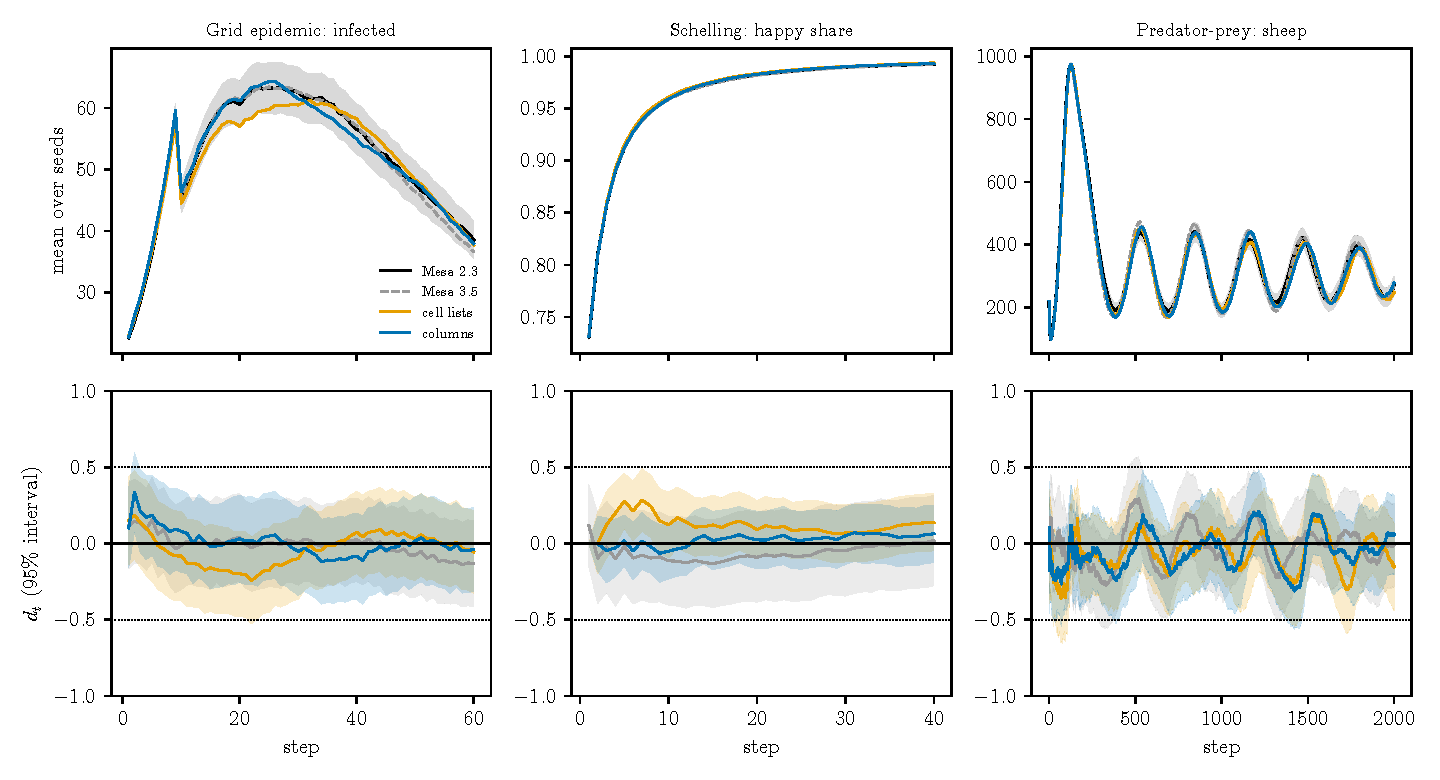
\includegraphics[width=\linewidth]{figures/trajectories_small}
  \caption{Top: the mean over 100 seeds of the infected count (grid epidemic), the happy
  share (Schelling) and the sheep count (predator-prey, 2,000 steps) for Mesa~2.3 (black,
  with a band of two standard errors), Mesa~3.5 (dashed) and the two \modelly{} variants.
  Bottom: the standardised paired difference $d_t$ from Mesa~2.3 at every step, with its
  95\% interval; dotted lines at $\pm 0.5$.}
  \label{fig:trajectories}
\end{figure}

\Cref{tab:trajectories} and \cref{fig:trajectories} give the results. On the curves, the
\modelly{} variants are as close to Mesa~2.3 as Mesa~3.5 is. On the grid epidemic's
infected curve the largest $|d_t|$ is 0.34 for the columns, 0.24 for the cell lists and
0.15 for Mesa~3.5 (upper bounds 0.54, 0.52 and 0.46), the largest relative difference of
the means over the steps where the epidemic is at least a tenth of its peak is 3.9, 7.4
and 5.3\%, one step of 60 has an interval excluding zero (the columns, at step 2, where
the first infections of the run are drawn), and no
permutation test finds a difference ($p = 0.16$, $0.52$, $0.92$). On Schelling's model the
columns follow Mesa~2.3 more closely than Mesa~3.5 does ($\sup_t |d_t| = 0.07$, upper
bound 0.29, against 0.13 and 0.46; the means of the happy share differ by at most 0.1\%)
while the cell lists show a small difference at steps 5 to 8 ($\sup_t |d_t| = 0.28$,
four steps with intervals excluding zero, permutation $p = 0.045$ for the happy share and
$0.048$ for the moves; at most 0.4\% of the happy share and 4.8\% of the moves). Over the
2,000 steps of predator-prey the largest $|d_t|$ is 0.29 to 0.39 for every implementation,
Mesa~3.5 included (upper bounds 0.61 to 0.67; a maximum over 2,000 noisy steps), the
permutation tests find nothing ($p \ge 0.24$), and the cycles of the four implementations
are in phase for 2,000 steps (\cref{fig:trajectories}): the same initial conditions set
the phase, and the period, 345 steps in Mesa~2.3, differs by at most 18 steps in the
others, with intervals of about $\pm 33$ steps.

On the scalars, 41 of the 52 \modelly{} comparisons are shown equivalent at their
prespecified margin (34 after the Holm correction) against 20 of 26 for Mesa~3.5 (17); the
study therefore does not establish equivalence for every quantity it tests, and we do not
claim that it does: 18 of the 52 are undecided at the familywise level. The
largest $|d|$ is 0.28 (Mesa~3.5: 0.18), and two paired $t$-tests of 52 fall below 5\% before
correction (none after; Mesa~3.5: none). The quantities not shown equivalent are the same
for every implementation, Mesa~3.5 included, and for the same reason: their margins are
narrower than what 100 seeds resolve. The peak's timing has a standard deviation of about
11 steps across seeds, so its paired interval is about $\pm 3.2$ steps against a margin of
$\pm 2$; the peak's height ($\pm 5\% = 3.8$ against an interval of $\pm 5.3$), the final
size ($\pm 14.6$ against $\pm 20$), the largest cluster ($\pm 1.9$ against $\pm 2.7$), the
total moves ($\pm 99$ against $\pm 110$, shown equivalent for the columns only) and the
period ($\pm 35$ against $\pm 33$) are the others. For all of these the point estimate lies
inside the margin, except the columns' peak timing, which is the one scalar shown different:
the columns' epidemic peaks $3.3$ steps earlier than Mesa~2.3's ($[-6.6, -0.1]$, $d =
-0.28$, 12\% of a mean of 28 steps); the cell lists' and Mesa~3.5's peak 2.9 and 2.1 steps
earlier with intervals that include zero. The second uncorrected difference is the cell
lists' share of residents with no same-kind neighbour, 0.4\% against 0.5\% ($d = -0.21$).
What the study does establish is this. Everything it was designed to catch beyond the
summary statistics agrees: the
cluster counts and mean cluster sizes are equivalent within $\pm 10\%$ for every
implementation after the Holm correction, the ten composition bins are equivalent within
0.02 for both \modelly{} variants before and after it (nine of ten for Mesa~3.5 after it),
the time to converge within 2 steps for every implementation before it, and the wolves die
out in 1 of 100 runs on Mesa~2.3 and Mesa~3.5 and in 0 of 100 on either \modelly{} variant
(sheep never), equivalent within 5 percentage points after it. The claim this supports
is bounded: on these three workloads, at this size, the faster forms follow the same
dynamics as Mesa~2.3 to within what 100 seeds resolve, and about as closely as Mesa~3.5 does;
for the six quantities whose margins 100 seeds cannot decide, the point estimates lie
within the margins but equivalence is not shown, and one timing difference is shown. The
variants are therefore not interchangeable for every scientific question: one whose answer
turns on the timing of an epidemic peak to within a few steps should treat the column form
as a different implementation and test it at its own tolerance. A run of this study at
the timed size, and on the other five playbooks, was not made; the three
chosen are the ones with spatial structure, a convergence process and a cycle.
